\documentclass[preview,border=7pt]{standalone}
\usepackage{amsmath,amssymb,xcolor}
\usepackage{tikz}
\usetikzlibrary{arrows.meta}
\definecolor{acc}{RGB}{47,143,132}
\definecolor{cyn}{RGB}{6,182,212}
\definecolor{amb}{RGB}{245,158,11}
\begin{document}
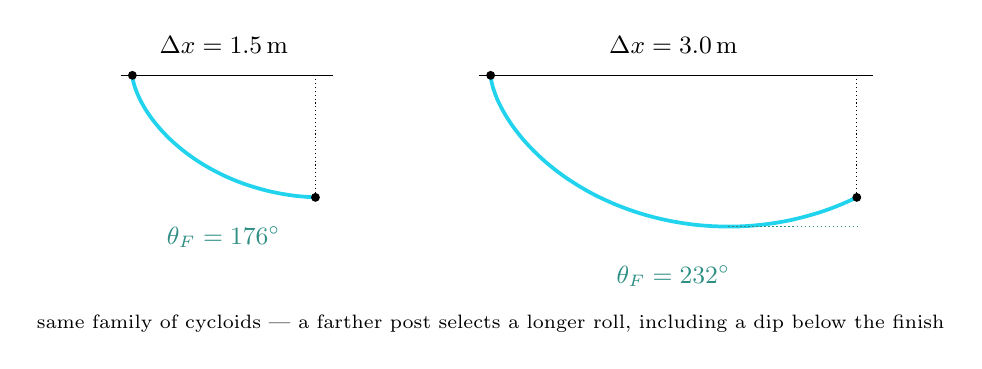
\begin{tikzpicture}
\definecolor{cycol}{RGB}{34,211,238}
% default Δx = 1.5 m, θ_F ≈ 176°
\begin{scope}[shift={(0,0)}]
\draw[line width=.45pt] (-0.15,0) -- (2.55,0);
\draw[cycol, line width=1.35pt] plot[smooth] coordinates {(0.000,0.000) (0.000,-0.000) (0.000,-0.000) (0.000,-0.000) (0.000,-0.000) (0.000,-0.000) (0.000,-0.000) (0.000,-0.000) (0.000,-0.000) (0.000,-0.001) (0.000,-0.001) (0.000,-0.001) (0.000,-0.002) (0.000,-0.003) (0.000,-0.003) (0.000,-0.005) (0.000,-0.006) (0.000,-0.007) (0.000,-0.009) (0.001,-0.012) (0.001,-0.014) (0.001,-0.017) (0.002,-0.021) (0.002,-0.025) (0.003,-0.029) (0.003,-0.035) (0.004,-0.040) (0.005,-0.047) (0.007,-0.054) (0.008,-0.062) (0.010,-0.071) (0.013,-0.081) (0.015,-0.092) (0.018,-0.103) (0.022,-0.116) (0.026,-0.130) (0.030,-0.145) (0.036,-0.161) (0.042,-0.179) (0.049,-0.197) (0.057,-0.217) (0.066,-0.239) (0.076,-0.261) (0.087,-0.286) (0.099,-0.311) (0.113,-0.338) (0.128,-0.366) (0.145,-0.396) (0.164,-0.427) (0.185,-0.460) (0.207,-0.494) (0.232,-0.529) (0.259,-0.566) (0.289,-0.604) (0.321,-0.643) (0.355,-0.683) (0.393,-0.724) (0.433,-0.766) (0.476,-0.809) (0.523,-0.852) (0.573,-0.896) (0.626,-0.940) (0.683,-0.985) (0.743,-1.029) (0.807,-1.073) (0.875,-1.117) (0.947,-1.160) (1.022,-1.202) (1.101,-1.243) (1.184,-1.283) (1.271,-1.321) (1.361,-1.357) (1.456,-1.391) (1.554,-1.422) (1.655,-1.451) (1.759,-1.477) (1.867,-1.499) (1.978,-1.518) (2.091,-1.533) (2.207,-1.543) (2.325,-1.550)};
\fill (0,0) circle (1.6pt);
\fill (2.325,-1.550) circle (1.6pt);
\draw[densely dotted, line width=.4pt] (2.325,0) -- (2.325,-1.550);
\node at (1.16,0.38) {\small $\Delta x=1.5\,\mathrm{m}$};
\node[acc] at (1.16,-2.05) {\small $\theta_F=176^\circ$};
\end{scope}
% Δx = 3.0 m, θ_F ≈ 232° — dips below the finish then climbs
\begin{scope}[shift={(4.55,0)}]
\draw[line width=.45pt] (-0.15,0) -- (4.85,0);
\draw[cycol, line width=1.35pt] plot[smooth] coordinates {(0.000,0.000) (0.000,-0.000) (0.000,-0.000) (0.000,-0.000) (0.000,-0.000) (0.000,-0.000) (0.000,-0.000) (0.000,-0.000) (0.000,-0.001) (0.000,-0.001) (0.000,-0.002) (0.000,-0.003) (0.000,-0.004) (0.000,-0.005) (0.000,-0.007) (0.000,-0.010) (0.001,-0.013) (0.001,-0.016) (0.001,-0.020) (0.002,-0.025) (0.003,-0.031) (0.003,-0.037) (0.005,-0.045) (0.006,-0.053) (0.008,-0.063) (0.010,-0.074) (0.012,-0.087) (0.016,-0.100) (0.019,-0.116) (0.024,-0.133) (0.029,-0.152) (0.035,-0.172) (0.043,-0.195) (0.051,-0.219) (0.061,-0.246) (0.072,-0.275) (0.085,-0.306) (0.100,-0.339) (0.117,-0.374) (0.136,-0.412) (0.158,-0.452) (0.182,-0.494) (0.209,-0.539) (0.240,-0.586) (0.273,-0.636) (0.311,-0.687) (0.352,-0.740) (0.397,-0.796) (0.447,-0.853) (0.501,-0.912) (0.560,-0.972) (0.624,-1.033) (0.693,-1.096) (0.768,-1.158) (0.849,-1.222) (0.935,-1.285) (1.028,-1.347) (1.126,-1.409) (1.231,-1.470) (1.342,-1.529) (1.460,-1.585) (1.583,-1.639) (1.713,-1.690) (1.848,-1.737) (1.990,-1.780) (2.137,-1.818) (2.289,-1.851) (2.446,-1.878) (2.607,-1.899) (2.773,-1.913) (2.942,-1.920) (3.113,-1.920) (3.286,-1.912) (3.461,-1.895) (3.637,-1.871) (3.812,-1.838) (3.985,-1.796) (4.157,-1.747) (4.326,-1.689) (4.490,-1.623) (4.650,-1.550)};
\fill (0,0) circle (1.6pt);
\fill (4.650,-1.550) circle (1.6pt);
\draw[densely dotted, line width=.4pt] (4.650,0) -- (4.650,-1.550);
\draw[acc, densely dotted, line width=.45pt] (3.018,-1.921) -- (4.650,-1.921);
\node at (2.32,0.38) {\small $\Delta x=3.0\,\mathrm{m}$};
\node[acc] at (2.32,-2.55) {\small $\theta_F=232^\circ$};
\end{scope}
\node at (4.55,-3.15) {\scriptsize same family of cycloids --- a farther post selects a longer roll, including a dip below the finish};
\end{tikzpicture}
\end{document}
